\documentclass[12pt]{article}
\usepackage[margin=1in]{geometry}
\usepackage{graphicx}
\usepackage{booktabs}
\usepackage{float}
\usepackage{amsmath}
\usepackage{hyperref}
\usepackage{fancyhdr}
\usepackage{caption}
\usepackage{pdflscape}
\usepackage{tikz} % Added TikZ package
\usepackage{xcolor} % Required for defining custom colors
\usetikzlibrary{positioning, arrows.meta, shapes.geometric} % Added TikZ libraries

% Set header and footer
\pagestyle{fancy}
\fancyhf{}
\fancyhead[L]{USC Facilities: Rain Barrel Water Pump System}
\fancyfoot[C]{\thepage}

\begin{document}

\title{
    \vspace{2in}
    \textbf{EMCH427-002} \\[1ex]
    \textbf{Product Architecture Report} \\[1ex]
    \textbf{Sponsor: USC Facilities} \\[1ex]
    \vspace{2in}
}

\author{
    \textbf{Team Members:} \\[2ex]
    Tanner Harmon - Designed 3D CAD models\\[1ex]
    Presston McConnell - Developed Unintended Interactions\\[1ex]
    William Wenzel - Developed Subsystem Clustering and Interactions\\[1ex]
    Jacob Vaught - Compilation, other work\\[2ex]
}

\date{}

\maketitle
\thispagestyle{fancy}

\newpage

% ------------------------------------------------------------
% Section 1: Introduction
% ------------------------------------------------------------
\section{Introduction}
\label{sec:introduction}

\begin{itemize}
    \item \textbf{Report Overview:}
    \begin{itemize}
        \item This report details the development of the product architecture for the Rain Barrel Water Pump System, which has been specifically designed for USC Facilities.
        \item It establishes a comprehensive framework that translates the conceptual design into a tangible physical form.
        \item The report ensures that all functional requirements of the system are met efficiently and effectively.
    \end{itemize}
    
    \item \textbf{Product Architecture Defined:}
    \begin{itemize}
        \item Product architecture serves as the blueprint for organizing the physical components of a product to perform their intended functions.
        \item It bridges the gap between the conceptual design phase and detailed engineering by outlining how various components interact within the system.
        \item This definition clarifies the roles and relationships of each component, ensuring seamless integration and functionality.
    \end{itemize}
    
    \item \textbf{Main Design Drivers:}
    \begin{itemize}
        \item \textbf{Sustainability:} The design aligns with USC's sustainability objectives by incorporating eco-friendly materials and energy-efficient processes.
        \item \textbf{Ease of Maintenance:} The system is designed to simplify servicing and part replacement, ensuring minimal downtime and reduced maintenance costs.
        \item \textbf{User Ergonomics:} Enhancing user interaction and experience is a priority, making the system intuitive and user-friendly.
        \item \textbf{Process Flow Efficiency:} The design optimizes the flow of operations within the system, ensuring smooth and efficient performance.
    \end{itemize}
    
    \item \textbf{Design Approach:}
    \begin{itemize}
        \item The project follows a structured approach inspired by best practices in engineering design, ensuring a methodical and effective development process.
        \item By prioritizing key factors such as sustainability, maintenance, ergonomics, and process flow, the design delivers a system that meets operational requirements comprehensively.
    \end{itemize}
\end{itemize}


\newpage
% ------------------------------------------------------------
% Section 2: Product Architecture Development
% ------------------------------------------------------------
\section{Product Architecture Development}
\label{sec:product_architecture}

The development of the product architecture encompasses several critical steps to ensure the system's functionality and efficiency. This section outlines the approach taken to translate the conceptual design into a detailed architectural framework.

\subsection{Modular versus Integrated Architecture}
\label{subsec:architecture_types}

A fundamental decision in product architecture development is the choice between modular and integrated architectures. 

\begin{itemize}
    \item \textbf{Modular Architecture:}
    \begin{itemize}
        \item In modular architecture, the system is divided into distinct modules or subsystems, each responsible for specific functions.
        \item Modules can be easily upgraded or replaced without affecting the entire system, enhancing flexibility and scalability.
    \end{itemize}
    
    \item \textbf{Integrated Architecture:}
    \begin{itemize}
        \item Integrated architecture involves designing the system as a cohesive unit with interdependent components.
        \item This approach can lead to optimized performance and reduced redundancy, as components are closely coordinated.
        \item However, it may result in increased complexity in development and maintenance, as changes in one component can impact others.
    \end{itemize}
\end{itemize}

Given the system's requirements and design drivers, a modular architecture has been adopted to enhance maintainability, scalability, and ease of upgrades.

\subsection{Component Layout}
\label{subsec:component_layout}

The component layout provides a spatial and functional representation of the system's elements and their clustering into subsystems. This layout is depicted in Figure \ref{fig:component_layout} and comprises the following aspects:

\begin{itemize}
    \item \textbf{Functional Elements:}
    \begin{itemize}
        \item Identification of all key components required for the system's operation.
        \item Definition of each component's role and interaction within the system.
    \end{itemize}
    
    \item \textbf{Clustering into Subsystems:}
    \begin{itemize}
        \item Grouping of related components into subsystems based on their functional relationships and proximity.
        \item Ensuring that each subsystem can operate independently while contributing to the overall system functionality.
    \end{itemize}
\end{itemize}

\begin{figure}[H]
    \centering
    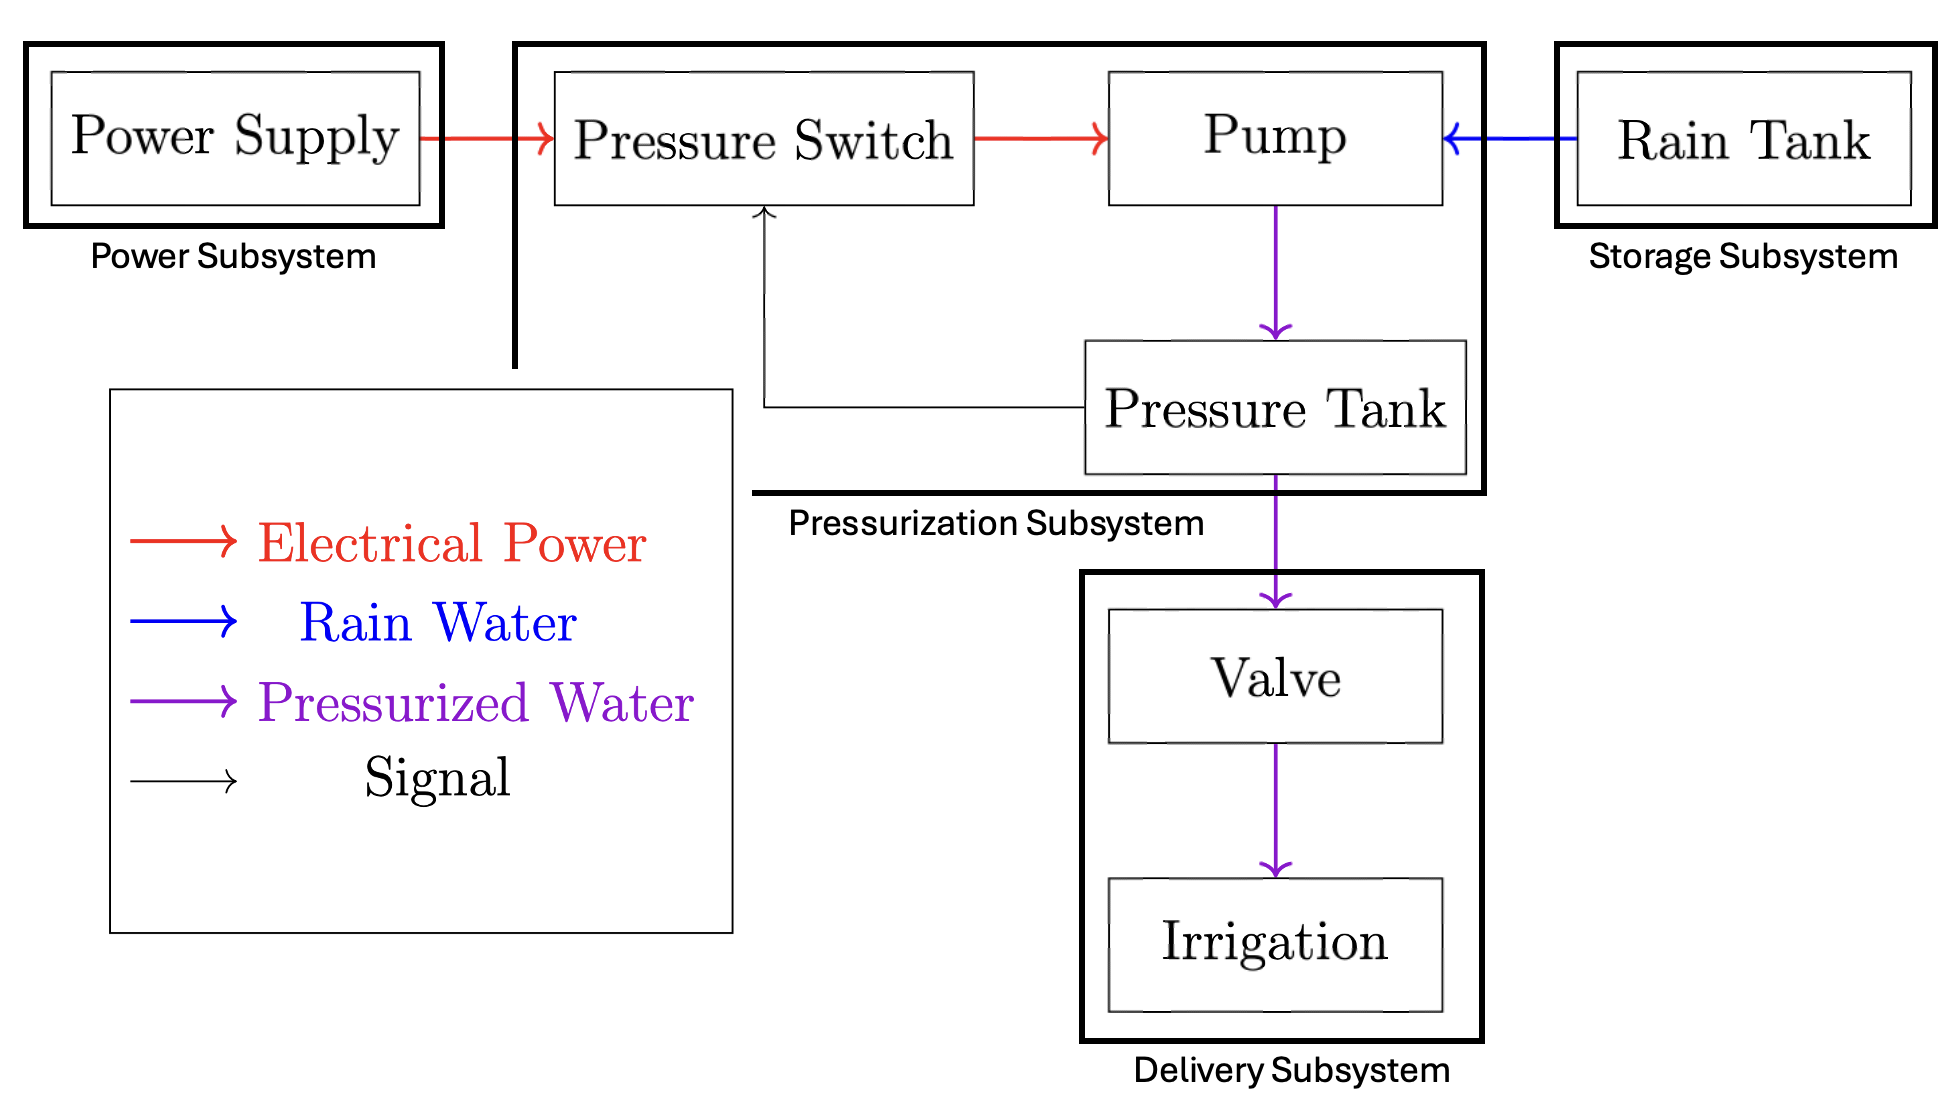
\includegraphics[width=1\textwidth]{component_layout.png}
    \caption{Component+Interaction Layout of the Rain Barrel Water Pump System}
    \label{fig:component_layout}
\end{figure}

\subsection{Clustering Rationale}
\label{subsec:clustering_rationale}

The clustering of components into subsystems was undertaken to enhance the system's modularity and maintainability. The following subsystems have been identified:

\begin{itemize}
    \item \textbf{Power Subsystem:}
    \begin{itemize}
        \item Comprises the power supply, including solar panels and batteries.
        \item Treated as a separate subsystem due to its provision of functional power and the presence of multiple components.
    \end{itemize}
    
    \item \textbf{Pressurization Subsystem:}
    \begin{itemize}
        \item Includes the pressure switch, pump, and pressure tank.
        \item Clustered together because these components operate in close proximity and are interdependent for maintaining system pressure.
    \end{itemize}
    
    \item \textbf{Storage Subsystem:}
    \begin{itemize}
        \item Consists of the rainwater tank.
        \item Managed as an independent subsystem to facilitate efficient water storage and easy access for maintenance.
    \end{itemize}
    
    \item \textbf{Delivery Subsystem:}
    \begin{itemize}
        \item Encompasses the valve and irrigation components.
        \item Grouped together as these are the primary points of user interaction for controlling water distribution.
    \end{itemize}
\end{itemize}

\subsection{Justification for Modular Architecture}
\label{subsec:justification_modular}

The decision to adopt a modular architecture was driven by several key factors:

\begin{itemize}
    \item \textbf{Sustainability:} Modular design allows for the integration of eco-friendly components and facilitates upgrades to more sustainable technologies without overhauling the entire system.
    \item \textbf{Ease of Maintenance:} By isolating components into distinct subsystems, maintenance tasks can be performed on individual modules without disrupting the entire system.
    \item \textbf{User Ergonomics:} The irrigation subsystem is designed for user interaction, and its separation ensures that user controls are easily accessible and manageable.
\end{itemize}

\newpage
\section{Interactions}
\label{sec:interactions}

Understanding the interactions within the Rain Barrel Water Pump System is crucial for optimizing performance and reliability. This section outlines both intended and consequential/incidental interactions, their impacts on architectural choices, identification of unintended interactions, and proposed solutions.

\subsection{Intended vs. Consequential/Incidental Interactions}

\begin{itemize}
    \item \textbf{Intended Interactions:}
    \begin{itemize}
        \item Planned exchanges of energy, materials, or information.
        \item Essential for the system's primary functions.
        \item Examples:
        \begin{itemize}
            \item Electrical power from the \textit{Power Subsystem} to the \textit{Pressurization Subsystem}.
            \item Water flow from the \textit{Storage Subsystem} to the \textit{Delivery Subsystem}.
            \item Control signals within the \textit{Pressurization Subsystem}.
        \end{itemize}
    \end{itemize}
    \item \textbf{Consequential/Incidental Interactions:}
    \begin{itemize}
        \item Unplanned secondary effects due to component proximity or arrangement.
        \item Can lead to performance issues or hazards if unaddressed.
        \item Examples:
        \begin{itemize}
            \item Heat generation from the pump affecting nearby components.
            \item Electromagnetic interference (EMI) from the pump motor.
            \item Mechanical vibrations causing wear or loosened connections.
        \end{itemize}
    \end{itemize}
\end{itemize}

\subsection{Impacts on Architectural Choices}

\begin{itemize}
    \item \textbf{Component Clustering:}
    \begin{itemize}
        \item Grouping interdependent components enhances efficiency.
        \item Increases risk of incidental interactions (e.g., heat buildup).
    \end{itemize}
    \item \textbf{Physical Placement:}
    \begin{itemize}
        \item Strategic positioning minimizes unintended interactions.
        \item Example: Locating the \textit{Power Subsystem} away from heat sources.
    \end{itemize}
    \item \textbf{Material Selection:}
    \begin{itemize}
        \item Choosing compatible materials prevents chemical reactions.
        \item Essential for longevity and safety.
    \end{itemize}
\end{itemize}

\subsection{Consequential Interaction and Solutions}

\begin{itemize}
    \item \textbf{Heat From Pump and BMS}
    \begin{itemize}
        \item Ensure adequate spacing between heat-generating and heat-sensitive components.
    \end{itemize}
    \item \textbf{Pump Vibrations}
    \begin{itemize}
        \item Mount the pump on vibration-dampening pads.
        \item Use flexible hoses or fittings to absorb vibrations.
        \item Perform regular maintenance checks.
    \end{itemize}
    \item \textbf{Leaking Connections}
    \begin{itemize}
        \item Utilize high-quality seals and fittings.
        \item Implement leak detection mechanisms.
        \item Protect electrical components with barriers or drip trays.
    \end{itemize}
    \item \textbf{Corrosion and degradation from weather}
    \begin{itemize}
        \item Use weatherproof enclosures for sensitive components.
        \item Select UV-resistant and corrosion-resistant materials.
        \item Apply protective coatings where necessary.
    \end{itemize}

\end{itemize}




\newpage
% ------------------------------------------------------------
% Section 2.3: Developing a Rough Geometric Layout
% ------------------------------------------------------------
\section{Geometric Layout}
\label{sec:geometric_layout}

A geometric layout is a spatial representation of the system's physical components, illustrating their sizes, shapes, and relative positions. It provides a visual understanding of how the components fit together within the available space, ensuring that the design is practical and meets spatial constraints.

The geometric layout of the Rain Barrel Water Pump System is shown in Figure~\ref{fig:geometric_layout_2d}. This layout was created using CAD software to approximate scale and includes the total dimensions (length, width, and height) of each component. The different subsystems are clearly labeled to correspond with their respective clusters.

\begin{figure}[H]
    \centering
    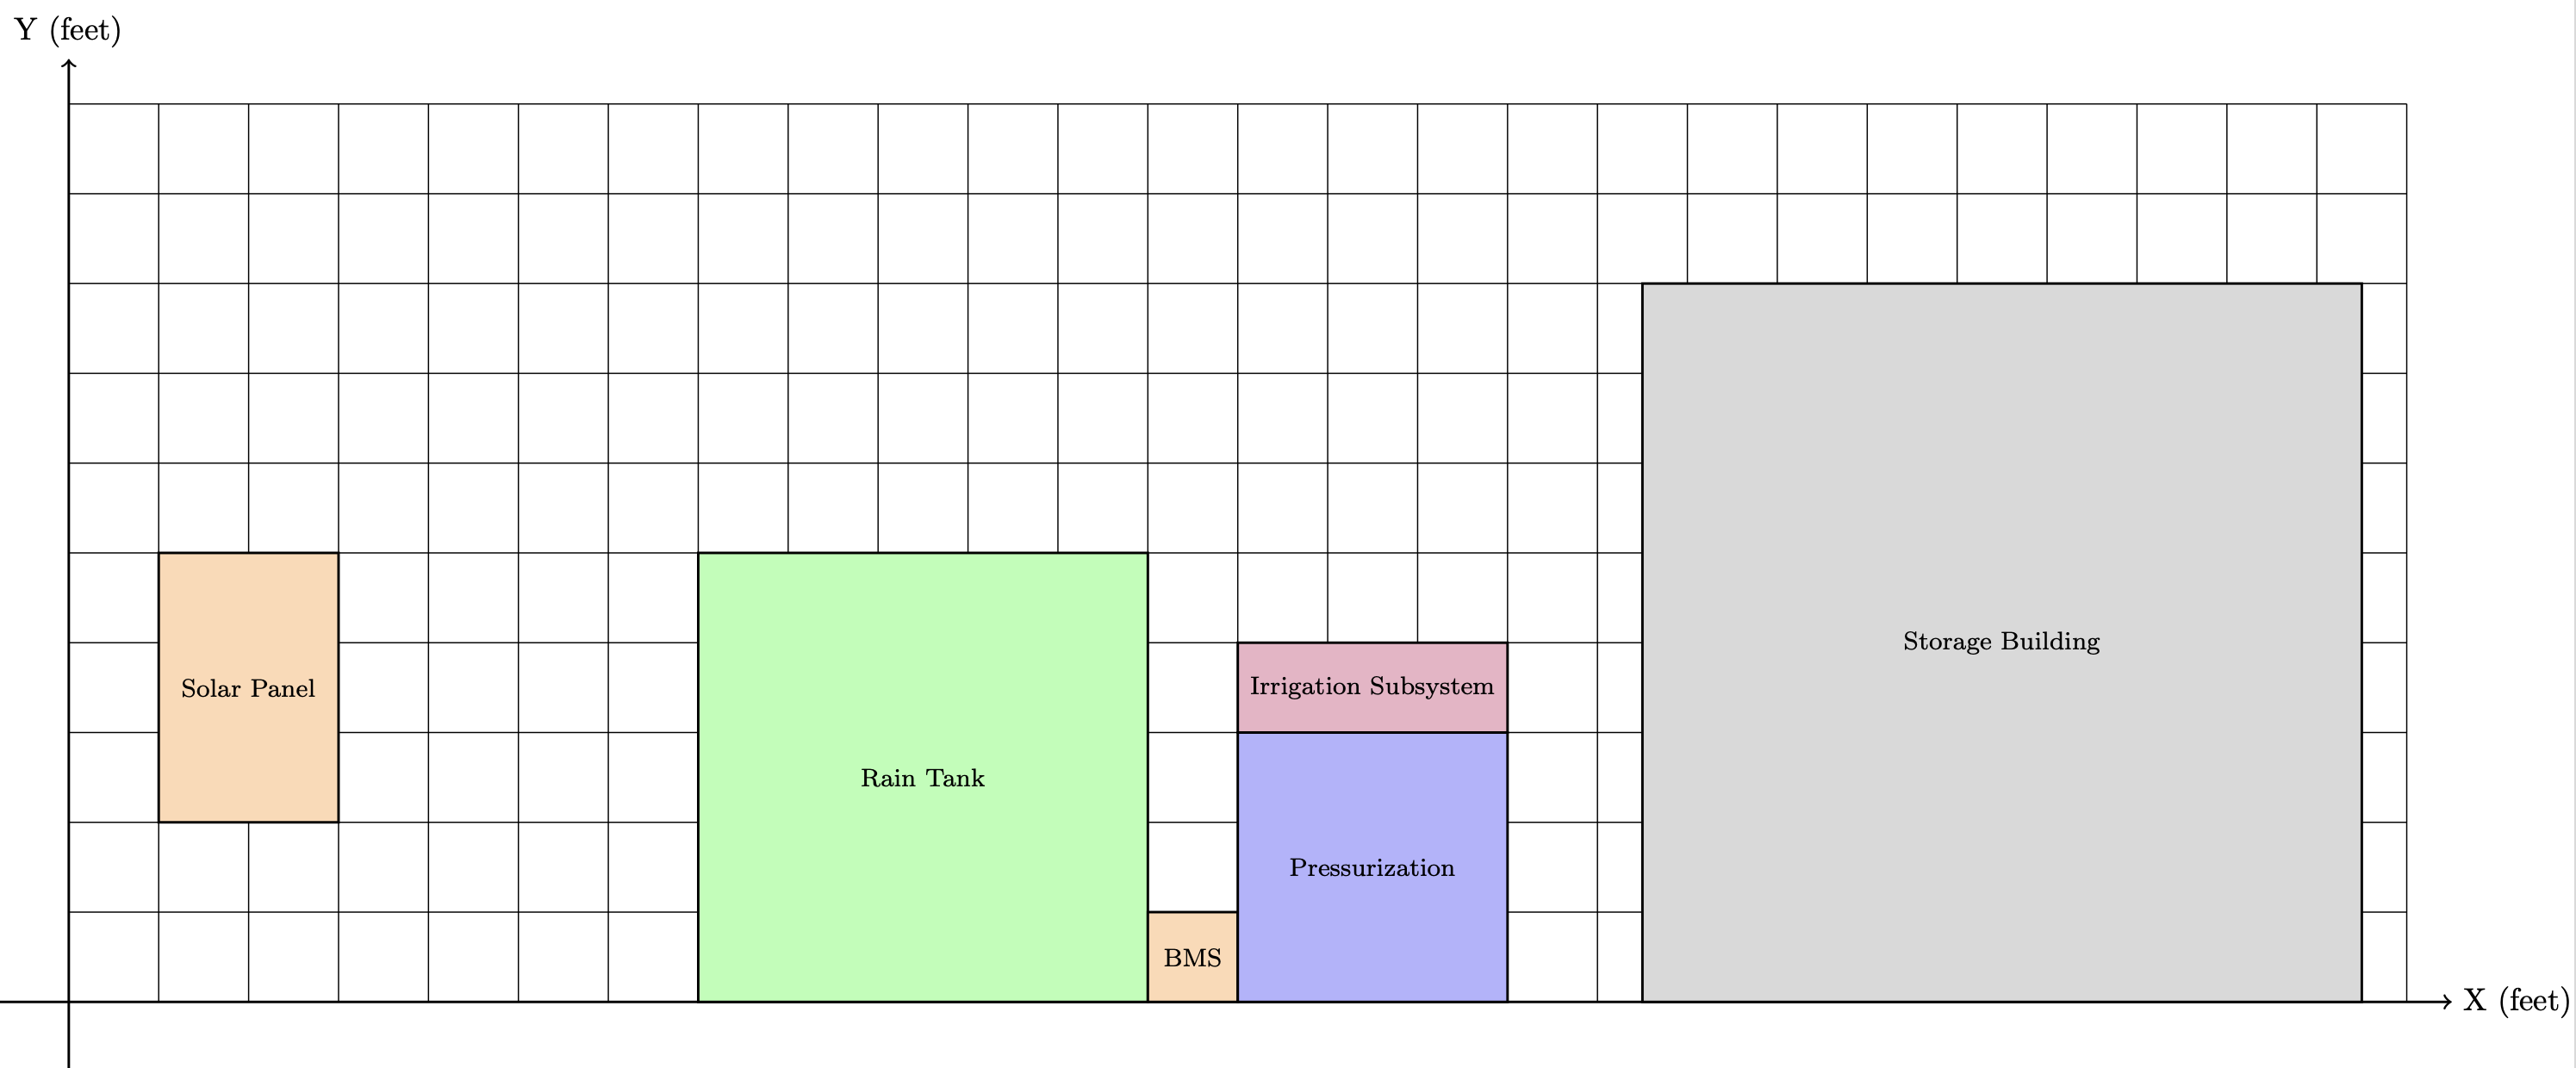
\includegraphics[width=\textwidth]{geometric_layout.png}
    \caption{2D Geometric Layout of the Rain Barrel Water Pump System}
    \label{fig:geometric_layout_2d}
\end{figure}

In the 2D layout, the existing storage building is included as it acts as a limiting factor for the placement of the system. The components and their dimensions (in feet) are as follows:

\begin{itemize}
    \item \textbf{Solar Panel:} 2 ft (L) $\times$ 3 ft (W) $\times$ 3 ft (H)
    \item \textbf{Rain Tank:} 5 ft (L) $\times$ 5 ft (W) $\times$ 7 ft (H)
    \item \textbf{Battery Management System (BMS):} 1 ft (L) $\times$ 1 ft (W) $\times$ 1 ft (H)
    \item \textbf{Pressurization Subsystem:} 3 ft (L) $\times$ 3 ft (W) $\times$ 3.5 ft (H)
    \item \textbf{Irrigation Subsystem:} 3 ft (L) $\times$ 1 ft (W) $\times$ 2 ft (H)
\end{itemize}

An additional 3D geometric layout is provided in Figure~\ref{fig:geometric_layout_3d}, offering a comprehensive visualization of the system's spatial arrangement and component dimensions.

\begin{figure}[H]
    \centering
    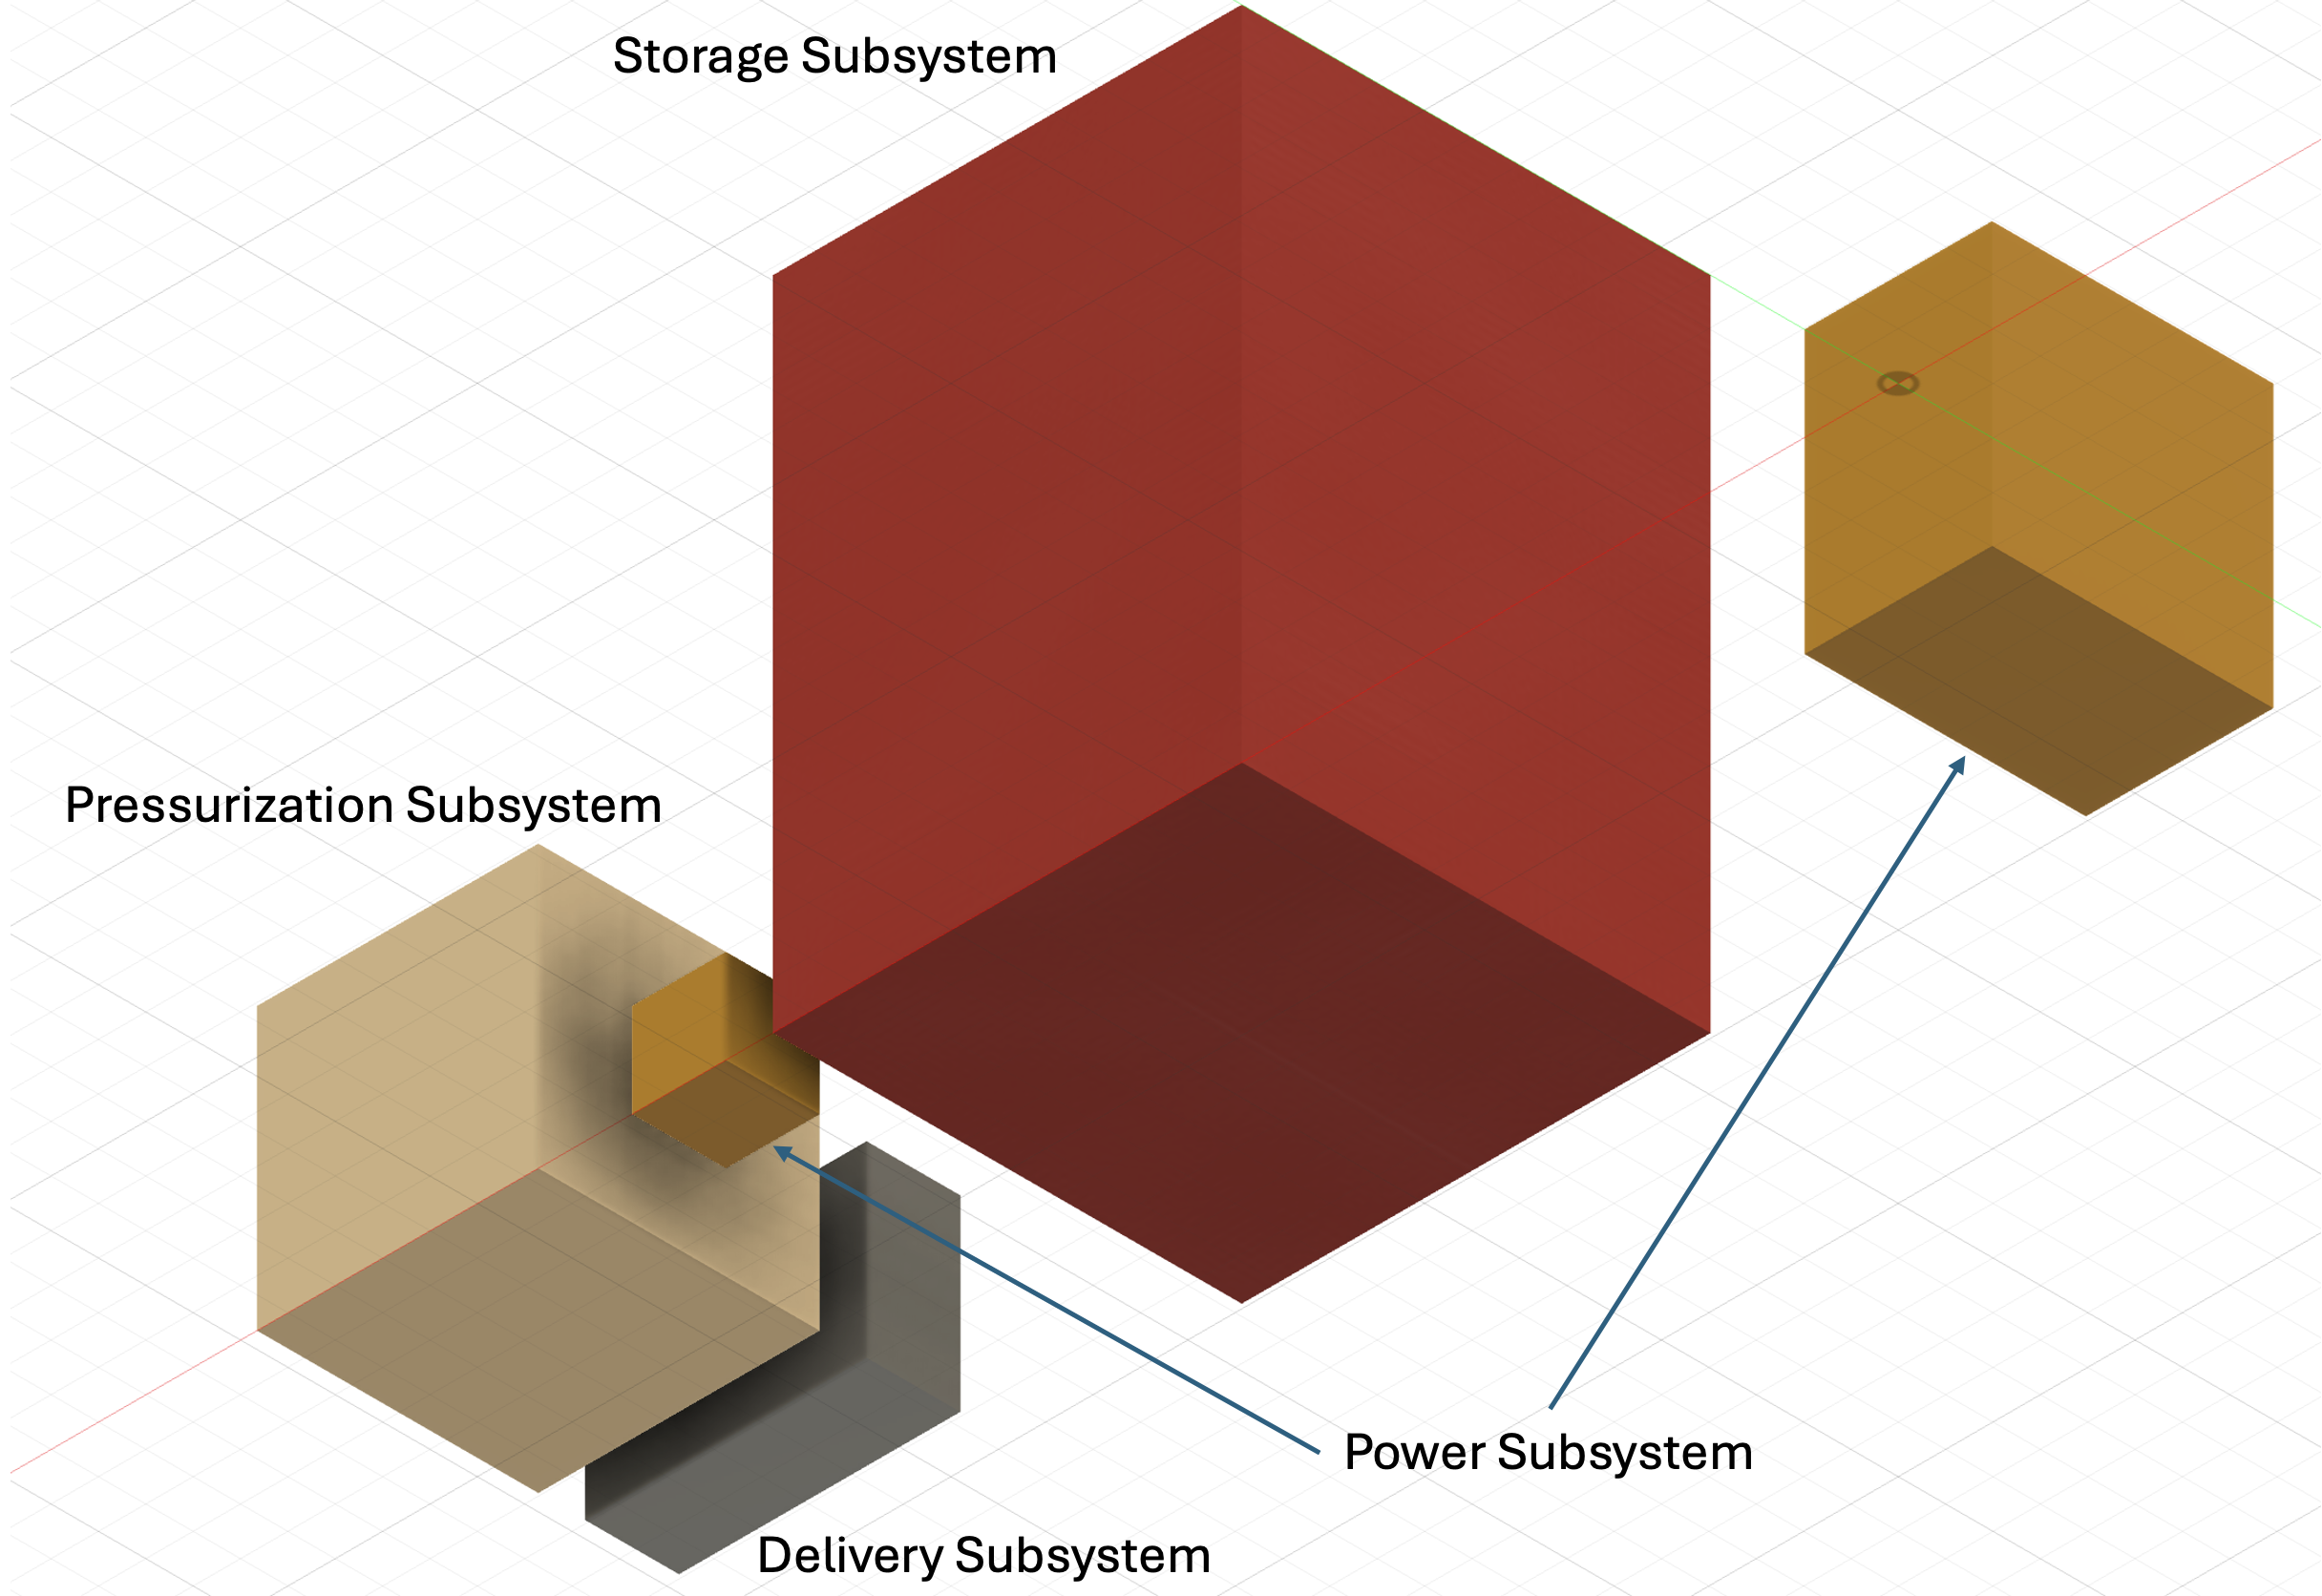
\includegraphics[width=0.8\textwidth]{3d_geometric_layout.png}
    \caption{3D Geometric Layout of the Rain Barrel Water Pump System}
    \label{fig:geometric_layout_3d}
\end{figure}

\subsection{Rationale for the Layout}

The layout decisions were guided by several key factors:

\begin{itemize}
    \item \textbf{Spatial Constraints:} The presence of the existing storage building limits the available space for system installation. Components are arranged to ensure they fit within this space without interfering with the building or other structures.

    \item \textbf{Maintainability:} Components requiring regular maintenance, such as the BMS and pressurization subsystem, are positioned for easy access. This facilitates servicing without the need to dismantle other parts of the system.

    \item \textbf{Interconnections and Interactions:} The layout minimizes unintended interactions between components. For example, the BMS is placed away from the pressurization subsystem to avoid exposure to moisture or heat that could affect its performance.

    \item \textbf{Compactness and Efficiency:} The overall system footprint is minimized by thoughtfully arranging components, which is essential given the spatial limitations imposed by the storage building.

\end{itemize}


% ------------------------------------------------------------
% Section 5: Conclusion
% ------------------------------------------------------------
\section{Conclusion}
\label{sec:conclusion}

The development of the product architecture for the Rain Barrel Water Pump System provides a solid foundation for detailed design and implementation. By systematically following established design steps and best practices, one will have:

\begin{itemize}
    \item Defined the functional elements and their relationships.
    \item Organized components into logical modules.
    \item Established a geometric layout that fits within spatial constraints.
    \item Identified and addressed interactions between modules.
\end{itemize}

The next phases will involve detailed design, including precise dimensions, tolerances, and material specifications, to bring the system from concept to reality.

% ------------------------------------------------------------
% Section 6: References
% ------------------------------------------------------------
\section*{References}
\begin{enumerate}
    \item Ulrich, K. T., \& Eppinger, S. D. (2016). \textit{Product Design and Development}. McGraw-Hill Education.
    \item Pahl, G., \& Beitz, W. (1996). \textit{Engineering Design: A Systematic Approach}. Springer.
\end{enumerate}

\end{document}
